\chapter{Deep RL con funciones Q}

\lecture{8}{2020-06-16}{DRL con funciones Q}

\section{Hacer funcionar Q-Learning con redes neuronales}%
\label{sec:hacer_funcionar_q_learning_con_redes_neuronales}

Al usar aproximadores de funciones se pierden las garantías de convergencia que se tienen en el
caso tabular. 

En el caso de \textit{online} Q-Learning, a parte de la demostración teórica de la no
convergencia, se tienen también los siguientes problemas:
\begin{itemize}
    \item La política inicial puede hacer que no se exploren algunos estados nunca.
    \item (Cierto parecido con la inestabilidad de las GAN)
    \item Con un batch de tamaño 1, la optimización es muy difícil.
    \item $y_i$ depende de  $Q_\phi$, por lo que el algoritmo no es exactamente
        descenso por gradiente. Para que fuese descenso por gradiente tendría que ser:
        \begin{align}
            \phi\gets\phi-\alpha \frac{dQ_\phi}{d\phi}
            (s_i,a_i)(Q_\phi(s_i,a_i)-r(s_i,a_i)+\gamma\max_{a'}Q_\phi(s'_i,a'_i))
        \end{align}
        Se puede ver que en algoritmo original los gradientes no 'fluyen' por la parte última
        de la ecuación. Para hacerlo, habría que optimizar el máximo (no lineal) y aún así no
        sería descenso por gradiente y no convergería (el profesor lo ha dicho).
        \item Las muestras no son i.i.d, ya que muestras sucesivas están relacionadas.
\end{itemize}

\subsection{Muestras relacionadas en \textit{online} Q-Learning}%
\label{sub:muestras_relacionadas_en_online_q_learning}

En el algoritmo original, lo que pasa es que se hace \textit{overfitting} de cada conjunto de
muestras que están relacionadas entre ellas, olvidando las muestras ya vistas
anteriormente.

Para resolver el problema:
\begin{itemize}
    \item Q-Learning paralelo sincronizado (como con Actor Critic). No resuelve el problema
        del todo. A diferencia de Actor Critic, Q-Learning es off-policy.
    \item \textit{Replay buffer}. Se tiene un dataset de transciciones creadas por una
        política y se entrena el modelo con esos datos. Esto consigue que las muestras no
        estén relacionadas entre ellas. También hace que el tamaño del batch sea mayor que 1.
        Cuando se llena el buffer se puede usar cualquier política, como por ejemplo una
        $\epsilon$-greedy de la política actual.
\end{itemize}

\begin{algorithm}
    \caption{Q-Learning con Replay Buffer}
    Crear dataset $\{(s_i,a_i,s_i',r_i)\}$ usando una política, añadirlo a $B$ \\
    \While{no se hayan hecho $K$ iteraciones}{
        Muestrear un batch de $B$ \\
$\phi \leftarrow \phi - \alpha \sum _ { i } \frac { d Q _ { \phi } } { d \phi } ( s _ { i } , a _
{ i } ) ( Q _ { \phi } ( s _ { i } , a _ { i } ) - [ r ( s _ { i } , a _ { i } ) + \gamma
\operatorname { max } _ { a ^ { \prime } } Q _ { \phi } ( s _ { i } ^ { \prime } , a _ { i } ^ {
\prime } ) ] )$
    }
\end{algorithm}

Normalmente se usa $K=1$, pero valores mas grandes de $K$ pueden ser más eficientes.

Todavía se tiene el problema de que no se está haciendo gradient descent real.

\subsection{Q-Learning con Target Networks}%
\label{sub:q_learning_con_target_networks}

Para lidiar con el problema de que no se está haciendo una regresión real, se cambia en el paso
3 del algoritmo anterior el $Q_\phi$ del final por $Q_\phi'$. Esto hace que ha no hayan
gradientes que tengan que 'fluir' por esa dirección y soluciona el problema. Evidentemente tiene
que cogerse una función  $Q_\phi'$ razonable por lo que se usa la política que se tenía hace
muchas iteraciones. Esto convierte el problema efectivamente en un problema de regresión
supervisada.

\begin{algorithm}
    \caption{DQN: Q-Learning con Target Networks y Replay Buffer}
    \label{alg:dqn}
    \While{se siga entrenando}{
        Guardar los parámetros de la red neuronal: $\phi'\gets\phi$\\
        \While{no se hayan hecho $N$ iteraciones}{
            Crear dataset $\{(s_i,a_i,s_i',r_i)\}$ usando una política, añadirlo a $B$ \\
            \While{no se hayan hecho $K$ iteraciones}{
                Muestrear un batch de $B$ \\
                $\phi \leftarrow \phi - \alpha \sum _ { i } \frac { d Q _ { \phi } } { d \phi } ( s _ { i } , a _
                { i } ) ( Q _ { \phi } ( s _ { i } , a _ { i } ) - [ r ( s _ { i } , a _ { i } ) + \gamma
                \operatorname { max } _ { a ^ { \prime } } Q _ { \phi } ( s _ { i } ^ { \prime } , a _ { i } ^ {
                \prime } ) ] )$
            }
        }
    }
\end{algorithm}

El algoritmo clásico DQN es una instanciación del algoritmo \ref{alg:dqn} donde $N=1$ y
$K=1$.

Esta es una solución heurística a un problema intratable por lo que no se consiguen las
garantías de covnergencia.

El target network se puede inicializar como se quiera pero una buena idea es hacerlo con pesos
pequeños para que la salida sea pequeña e influya más la recompensa en las etapas iniciales.

Esta técnina puede parecer que sea muy brusca en los cambios $\phi'\gets\phi$,
por lo que se puede utilizar una promediación de Polyak cada vez que se actualice $\phi$:
\begin{align}
    \phi':\phi&'\gets\tau\phi'+(1-\tau)\phi & \tau&=0.999 \textrm{ funciona bien }
\end{align}


\section{Una vista generalizada de los algoritmos Q-Learning}%
\label{sec:una_vista_generalizada_de_los_algoritmos_q_learning}

Se puede ver DQN como Fitted Q-Learning pero del revés. Ambos son dos formas de expresar el mismo
proceso:

\begin{figure}[htpb]
	\centering
	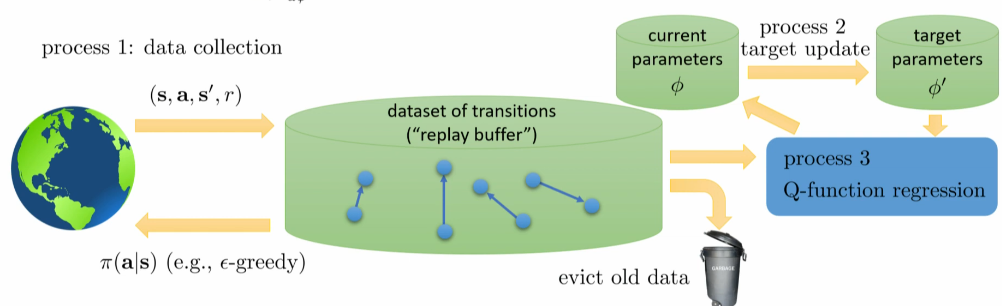
\includegraphics[width=0.8\linewidth]{figures/2020-06-16-174411_1002x306_scrot.png}
	\caption{Vista general de Q-Learning. El proceso 1 es la obtención del Replay Buffer, que
    puede ser implementado con una FIFO, ya que se llenará de datos y habrá que ir vaciándola. El
proceso 2 es la actualización de la Target Network, que puede ser repentina cada ciertos pasos o
continuada con la promediación de Polyak. El proceso 3 es la regresión. }
\label{fig:qlearn}
\end{figure}

\begin{itemize}
    \item 
        El algoritmo Online Q-Learning explicado en el tema anterior es un caso particular de
        esta vista general en el cual los datos se eliminan conforme llegan y los 3 procesos corren a la
        misma velocidad.
    \item DQN: los procesos 1 y 3 van a la misma velocidad y el proceso 2 es más lento. El tamaño
        del buffer es mayor que 1.
    \item Fitted Q-Iteration: el proceso 3 está en el interior del bucle del proceso 2, el cual a
        su vez está en el interior del proceso 1.
\end{itemize}

Se puede acelerar el proceso de aprendizaje si se usa un Prioritized Replay Buffer. En el cual
se eligen con más probabilidad las muestras que hacen que se genere el mayor error. 

\section{Trucos prácticos para mejorar Q-Learning}%
\label{sec:trucos_prácticos_para_mejorar_q_learning}

\subsection{¿Son los valores Q precisos?}%
\label{sub:_son_los_valores_q_precisos_}

La función Q es una función numérica con significado: la esperanza de la recompensa si
empiezas en un estado, tomas una acción y sigues con la política $\pi$. La pregunta es si las
redes neuronales aprenden los valores de estas predicciones.

\begin{figure}[H]
	\centering
	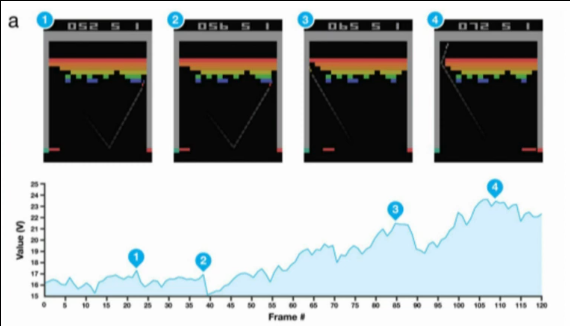
\includegraphics[width=0.5\linewidth]{figures/2020-06-16-180133_570x326_scrot.png}
    \caption{En este gráfico se pueden ver los máximos locales de Q cuando el algoritmo piensa
    que está en un buen estado. Se puede ver que el mayor de estos máximos es cuando rompe la
barrera.}
\label{fig:breakout}
\end{figure} 

Esto parece razonable, pero ¿son numéricamente precisos?

\begin{figure}[H]
	\centering
	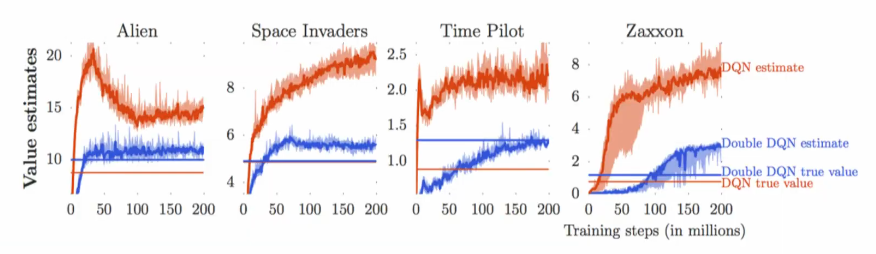
\includegraphics[width=0.8\linewidth]{figures/2020-06-16-180346_876x254_scrot.png}
    \caption{(Ingorar por ahora las líneas azules) Se puede ver que las estimaciones de DQN
    son mayores que la recompensa real obtenida (lineas rojas horizontales).}
    \label{fig:estimaciones}
\end{figure}

Se ve que todos los números son muy grandes, DQN es muy 'optimista'. Una intuición de por qué
esto pasa es la siguiente: los valores Q estimados vienen con mucha varianza (ruido), por lo que
al aplicar el operador máx, se están quedando con esos valores máximos que realmente son ruido.

Más concretamente, el target-value se calcula:
\begin{align}
y _ { j } = r _ { j } + \gamma \operatorname { max } _ { a _ { j } ^ { \prime } } Q _ { \phi ^ { \prime } } ( s _ { j } ^ { \prime } , a _ { j } ^ { \prime } )
\end{align}

El término máx es el problema. Imaginemos que tenemos dos variables aleatorias $X_1$ y
$X_2$ (se puede pensar que son valores Q para dos acciones distintas). Se puede demostrar que:
\begin{align}
E [ \operatorname { max } ( X _ { 1 } , X _ { 2 } ) ] \geq \operatorname { max } ( E [ X _ { 1 } ] , E [ X _ { 2 } ] )
\end{align}

Lo que significa que si se maximizan estas variables, siempre se coge la mayor + el ruido.
Por lo que da un valor siempre mayor que la esperanza de estos valores. $Q_{ \phi' }(s',a')$ no
es perfecta (se 've' con ruido). Por lo que  $\max_{a'}Q_{\phi'}(s',a')$ está sobreestimando
el siguiente valor. Otra manera de pensarlo es escribirlo de esta manera:
\begin{align}
    \label{eq:argmax}
Q _ { \phi ^ { \prime } } ( s ^ { \prime } , a ^ { \prime } ) = Q _ { \phi ^ { \prime } } ( s ^ { \prime } , \operatorname { arg } \operatorname { max } _ { a ^ { \prime } } Q _ { \phi ^ { \prime } } ( s ^ { \prime } , a ^ { \prime } ) )
\end{align}
Por lo que si se escoge la acción que maximiza $Q_{\phi'}$ y resulta que esa acción tiene un
valor Q erróneamente alto por culpa del ruido, se estará sobreestimando su valor.

\subsection{Double Q-Learning}%
\label{sub:double_q_learning}

El problema viene de que el mismo ruido afecta al argmax y a $Q_{\phi'}$. Por lo que si el
ruido aplicado a ambos se decorrelase, el problema se solucionaría. Para conseguir esto se
pueden usar dos redes neuronales (cada una con su ruido correspondiente pero no relacionados
entre ellos): una para elegir la acción y otra para evaluar el valor:
\begin{align}
Q _ { \phi _ { A } } ( s , a ) \leftarrow r + \gamma Q _ { \phi _ { B } } ( s ^ { \prime } ,
\operatorname { arg } \operatorname { max } _ { a ^ { \prime } } Q _ { \phi _ { A } } ( s ^ {
\prime } , a ^ { \prime } ) )\\
Q _ { \phi _ { B } } ( s , a ) \leftarrow r + \gamma Q _ { \phi _ { A } } ( s ^ { \prime } , \operatorname { arg } \operatorname { max } _ { a ^ { \prime } } Q _ { \phi _ { B } } ( s ^ { \prime } , a ^ { \prime } ) )
\end{align}

No hace falta aplicar muchos cambios a los algoritmos que ya se han deducido anteriormente en el
tema ya que se tiene $Q_\phi$ y  $Q_{\phi'}$. Por lo que el único cambio que habría que hacer
sería cambiar:
\begin{align}
y = r + \gamma Q _ { \phi ^ { \prime } } ( s ^ { \prime } , \operatorname { arg } \operatorname { max } _ { a ^ { \prime } } Q _ { \phi ^ { \prime } } ( s ^ { \prime } , a ^ { \prime } ) )
\end{align}
por:
\begin{align}
y = r + \gamma Q _ { \phi ^ { \prime } } ( s ^ { \prime } , \operatorname { arg } \operatorname { max } _ { a ^ { \prime } } Q _ { \phi } ( s ^ { \prime } , a ^ { \prime } ) )
\end{align}

Esto no es del todo correcto ya que ambas redes no son del todo independientes, pero
en la práctica están lo suicientemente decorreladas para que funcione.

En la práctica, el problema de los valores sobreestimados no es tan malo, pero solucionarlo
nos lleva a políticas ligeramente mejores.

Se puede ver el efecto de Double Q Learning en la figura \ref{fig:estimaciones} (color
azul).

\subsection{Multi-step returns}%
\label{sub:multi_step_returns}

Consiste en desenrollar la función de Bellman. La intuición es que si en el estado actual no se
tiene una buena estimación, se puede ir más rápido a un valor cercano si se miran las
recompensas más cercanas (parecido al caso de actor-critic en la sección
\ref{sec:elegibility_traces_y_n_step_returns}). Por lo que el targuet queda como:

\begin{align}
    y _ { j , t } = \sum _ { t ^ { \prime } = t } ^ { t + N - 1 } \gamma^{t'-t}r _ { j , t ^ { \prime } } + \gamma ^ { N } \operatorname { max } _ { a _ { j , t + N } } Q _ { \phi ^ { \prime } } ( s _ { j , t + N } , a _ { j , t + N } )
\end{align}

Cuando ya se tenga un valor bastante aproximado, valores altos de $N$ introducirán más
varianza por lo que hay que jugar con el valor. Normalmente se usan valores entre 4 y 10.

La desventaja es que las recompensas vienen de una trayectoria, lo que hace que el modelo deje
de ser \textit{off-policy}.

Para solucionar este problema se puede hacer lo siguiente:
\begin{itemize}
    \item Ingorarlo (para valores pequeños de $N$ (como por ejemplo 4)) suele funcionar
        bien.
    \item Cortar la traza: seleccionar $N$ adaptativamente. Por ejemplo si se está jugando a
        Atari (dimensiones del espacio de acciones bajo) puede ser que durante varios pasos
        se elija la misma acción y se pueden meter en un batch.
    \item Importance Sampling
\end{itemize}

\section{Métodos Q-Learning contínuos}%
\label{sec:métodos_q_learning_contínuos}

Para el caso discreto, escoger la acción que maximiza Q es trivial. En el caso contínuo, hay
varias opciones para aproximar la maximización.

La maximización ocurre en el bucle interno del algoritmo por lo que se quiere evitar que la
optimización sea cara computacionalmente.

\begin{itemize}
    \item Opción 1: optimización
        \begin{itemize}
            \item correr SGD con respecto a $a$. No es una buena idea porque es lento.
            \item Si el espacio de acciones tiene una dimensionalidad baja, se puede usar
                optimización estocástica (Monte Carlo: coger aleatoriamente varias $a$ y coger
                la mayor, por ejemplo). Una solución más precisa es usar
                \textit{Cross-Entropy Method (CEM)}. Consiste en muestrear unas cuantas
                acciones, evaluar sus valores y en vez de coger la que tenga el mayor valor, se
                crea una distribución en las mejores obtenidas y se muestrean acciones
                de esa distribución, repitiendo el proceso. También se pueden aplicar otros
                algoritmos como CMA-ES. Estos métodos funcionan para espacios de acciones
                de dimensionalidad menor que 40.
        \end{itemize}
    \item Opción 2: usar una clase de funciones que sean fáciles de optimizar. En vez de
        usar una red neuronal, se puede por ejemplo aproximar los valores Q con una función
        cuadrática. En el caso de que se tenga un espacio de estados muy complejo, se puede
        crear una arquitectura que sea cuadrática en las acciones pero no lineal en los
        estados:
\begin{figure}[H]
	\centering
	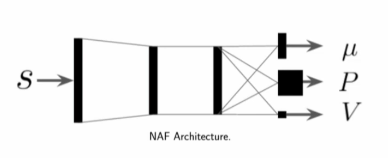
\includegraphics[width=0.4\linewidth]{figures/2020-06-16-185156_388x158_scrot.png}
\end{figure}
        \begin{align}
Q _ { \phi } ( s , a ) = - \frac { 1 } { 2 } ( a - \mu _ { \phi } ( s ) ) ^ { T } P _ { \phi } ( s ) ( a - \mu _ { \phi } ( s ) ) + V _ { \phi } ( s )
        \end{align}
        La acción que da el mayor valor es $\mu$. Esta arquitectura se llama NAF
        )(\textit{Normalized Advantage Functions}). Como ventajas tiene que no cambia el
        algoritmo y es tan eficiente como Q-Learning, pero a costa de perder poder de
        representación. Se aplica solo en casos en que el espacio de acciones sea muy
        sencillo.
    \item Opción 3: entrenar otra red neuronal que prediga la acción que optimice el valor.
        Un algoritmo de esta categoría sería DDPG (\textit{Deep Deterministic Policy
        Gradients}). En la publicación del algoritmo los autores lo describen como un
        método Actor-Critic pero realmente se puede ver como una aproximación de
        Q-Learning.\\\\Partiendo de la ecuación \ref{eq:argmax} se puede ver que el problema está
        en calcular el argmax de $a$. Por lo que se podría entrenar a una red neuronal para
        que aproxime este valor: 
         \begin{align}
             \mu_\theta(s) \approx arg\max_a Q_\phi(s,a)
        \end{align}
        Para entrenar a esta red neuronal, simplemente se tiene que resolver $\theta \gets
        arg\max_\theta Q_\phi(s,\mu_\theta(s))$. Mediante la regla de la cadena se puede ver
        que $\frac{dQ_\phi}{d\theta} = \frac{da}{d\theta}\frac{dQ_\phi}{da}$ 
        (un paquete de diferenciación automática hace esto automáticamente). Ahora cuando se
        calculen los target-values, en vez de usar argmax, se usa $\mu_\theta$:
        \begin{align}
y _ { j } = r _ { j } + \gamma Q _ { \phi ^ { \prime } } ( s _ { j } ^ { \prime } , \mu _ { \theta } ( s _ { j } ^ { \prime } ) ) \approx r _ { j } + \gamma Q _ { \phi ^ { \prime } } ( s _ { j } ^ { \prime } , \operatorname { arg } \operatorname { max } _ { a ^ { \prime } } Q _ { \phi ^ { \prime } } ( s _ { j } ^ { \prime } , a _ { j } ^ { \prime } ) )
        \end{align}

        \begin{algorithm}
            \caption{DDPG}
            \label{alg:ddpg}
            \While{se siga entrenando}
            {
                Tomar una acción $a_i$ y observar $(s_i,a_i,s_i',r_i)$, añadirlo a  $B$ \\
                Muestrear un mini-batch de $\{s_j,a_j,s'_j,r_j\}$ de  $B$ de manera uniforme.\\
                Calcular $y_j=r_j+\gamma Q_{\phi'}(s'_j,\mu_{\theta'}(s_j'))$
                usando  $Q_{\phi'}$ y $\mu_{\theta'}$\\
                $ \phi \leftarrow \phi - \alpha \sum _ { j } \frac { d Q _ { \phi } } { d \phi } ( s
                _ { j } , a _ { j } ) ( Q _ { \phi } ( s _ { j } , a _ { j } ) - y _ { j } ) $\\
                $ \theta \leftarrow \theta + \beta \sum _ { j } \frac { d \mu } { d \theta } ( s _ {
                j } ) \frac { d Q _ { \phi } } { d a } ( s _ { j } , a ) $\\
                Actualizar $\phi'$ y  $\theta'$ (por ejemplo con Polyak)
            }
        \end{algorithm}

        Se podría entrenar $\mu_\theta$ hasta la convergencia, pero Q está cambiando
        constantemente, por lo que se tiene que ir actualizando.
\end{itemize}

\section{Consejos prácticos para Q-Learning}%
\label{sec:consejos_prácticos_para_q_learning}

Es buena idea empezar en tareas sencillas primero, ya que el algoritmo no es muy estable. Puede
tardar mucho en aprender.

Replay Buffers grandes ayudan a mejorar la estabilidad.

Es recomendable empezar con una alta exploración ($\epsilon$).

Los errores de Bellman pueden hacer que los gradientes sean grandes, por lo que se deben cortar
los gradientes o usar \textit{Huber loss} (como MSE en el origen pero lineal lejos del origen).

Usar Double Q Learning, ayuda mucho y es muy sencillo.

N-Steps ayuda pero tienen sus inconvenientes.

Testear los modelos con varias semillas aleatorias, ya que los resultados pueden variar mucho.
